\chapter{Literature review}
\label{ch:Literature review}
\section{Analysis-based tools for engineers}
The development of finite element analysis (FEA) has resulted in many different, but very similar, software analysis tools. These tools are often too complex and not agile enough to be used for conceptual design. Their use requires a high level of skills both in connection with the software and in engineering terms. This type of software has been developed for the late design stage as a tool for the engineer to verify the form. 

 The analysis procedure for this type of software is often a step-by-step workflow, where all the steps need to be completed in order before the analysis is carried out, see Figure \ref{fig:conventional-cycle}. The user experience has been compromised by this step-by-step evolution.

\begin{figure}
  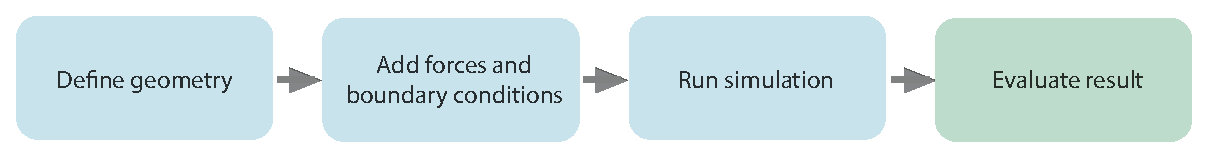
\includegraphics[width=310pt]{graphics/conventional-cycle.eps}
  \caption{Conventional simulation cycle}
  \label{fig:conventional-cycle}
\end{figure}

\begin{figure}
  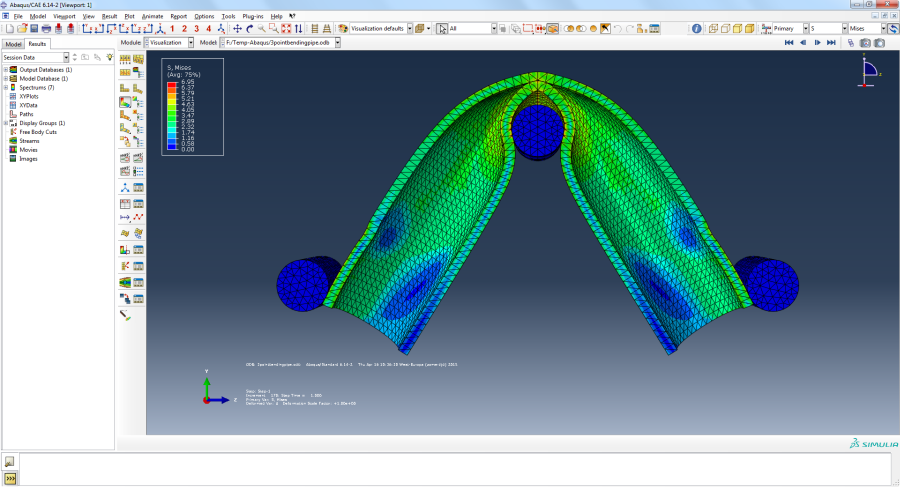
\includegraphics[width=350pt]{graphics/abaqus.png}
  \caption{User interface of conventional analysis software (ABAQUS)}
  \label{fig:abaqus}
\end{figure}

\section{Geometry-based tools for architects}
\subsection{History}
\begin{figure}
  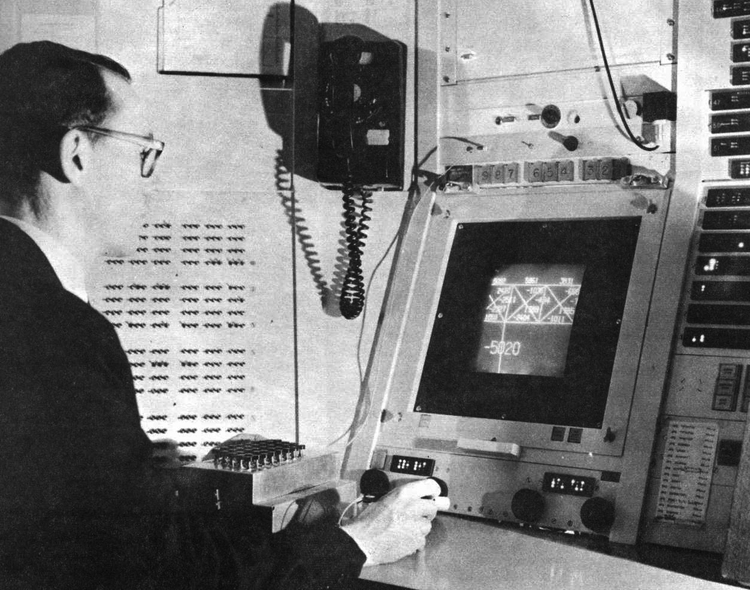
\includegraphics[width=350pt]{graphics/sketchpad.jpg}
  \caption{Sketchpad - the first CAD tool}
  \label{fig:sketchpad}
\end{figure}
The first computer-aided design (CAD) tool, termed Sketchpad \cite{Aish2005}, was developed by Ivan Sutherland at MIT in 1963. The revolutionary feature of Sketchpad was real-time representation of the geometry on the display, which could be modified with the use of a new input device, a light pen. The light pen enabled a complete interaction loop between the computer and the designer. The software had support for complex relationships between graphical elements; for example, a line could be defined by relationship to other graphical objects, perpendicular to, parallel to, same length etc. Sutherland had a vision that the designer would first create a rough sketch of the design. And then, as the design matured, apply constraints to the graphical objects to get a more detailed and precise design. 

Computer aided design tools, 2D drafting tools, were first affordable and accessible to a wider audience in the 1980s \cite{Aish2005}. The succeeding 2D drafting software unfortunately failed to capture Sutherland’s original intentions of using the computer as a creative design tool, by not including the constraint model. 

\subsection{Present day}
As mentioned earlier, many different geometric modeling tools are today available for designers, such as parametric modelers. These parametric modelers have successfully captured some of Sutherland’s ideas of constraint models. 

The software Rhinoceros 3D \cite{Rhino}, which is a NURBS modeler, can be combined with the plug-in Grasshopper \cite{Grasshopper}, that enables a visual programming environment. The software developer company Autodesk has also launched a parametric modeling tool named Dynamo \cite{Dynamo} that has similar features.


In Grasshopper the designer can connect a slider to a parameter - for example the width or curvature of a model – the geometry then updates in real-time as sliders are manipulated. This enables complex shapes and forms to be generated and manipulated, allowing the designer to explore the parametric design space. 

Many plug-ins also exist for Grasshopper, and these can be combined with each other, one such example is Karamba \cite{Karamba}, which enables structural performance feedback within the parametric modeler. 

\section{Existing conceptual design tools}

\textit{''Geometry and algorithms can exist in the abstract, but to be of any practical significance, to become a design tool which can be used by designers, then these have to be encapsulated in an executable form, as working software…''} - Robert Aish \cite{Shea2005}

A number of different conceptual design tools exist; they have here been divided into categories depending on the computational methods that they make use of.

\subsection{Real-time analysis tools}

\begin{figure}
  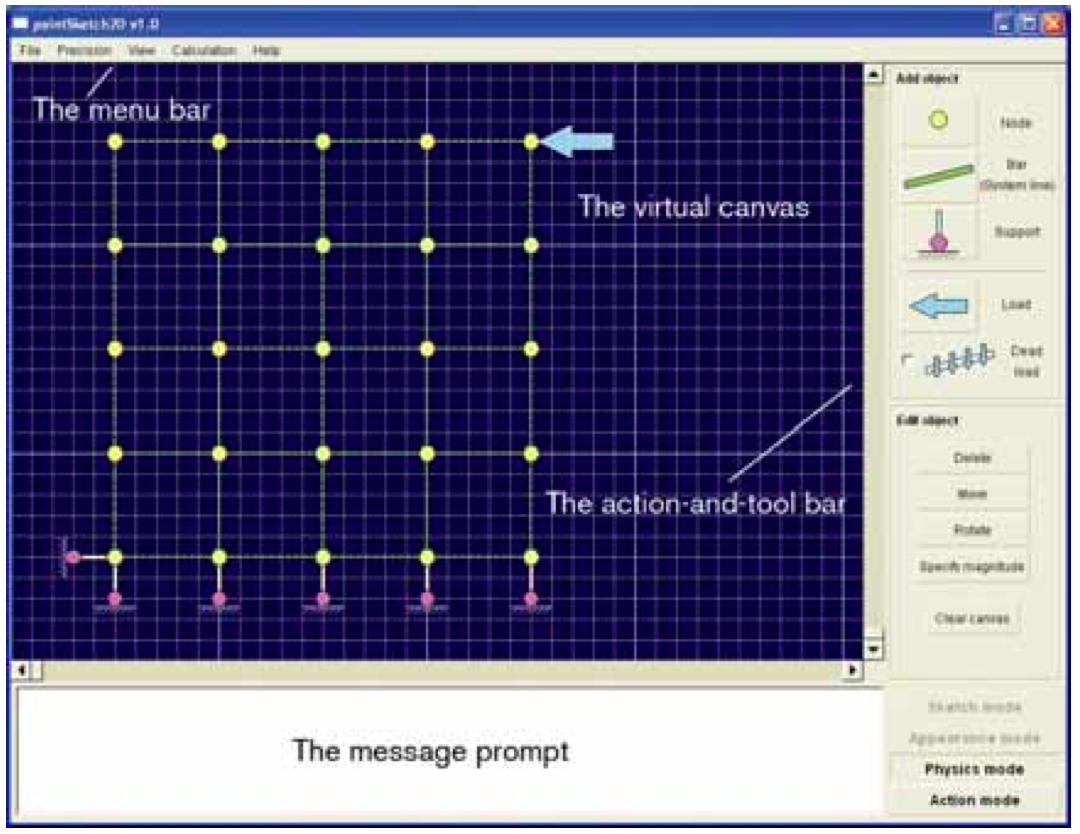
\includegraphics[width=350pt]{graphics/pointsketch.png}
  \caption{The software tool PointSketch}
  \label{fig:pointsketch}
\end{figure}

This type of conceptual design tools makes use of simple mathematical models to provide the user real-time feedback from structural analysis. Various such tools have previously been developed, the first two such tools were developed in parallel and released in 2006, named Pointsketch \cite{Olsson2006} (see Figure \ref{fig:pointsketch}) and Arcade \cite{martini2008new}. In the two different software tools, the user can create a structural model using mouse and keyboard input. Forces can then be applied to the model and the results are visualized in real-time 

The first tools were developed in academia but industry has shown interest in the concept. Autodesk launched a new application in 2011 named ForceEffect \cite{Autodesk2011}, which is available both as an tablet and as a web application. The application is developed for designers to analyze and visualize two-dimensional truss structures. The tablet application utilizes a direct manipulation user interface style where the user can make changes to the model by directly touching the objects. The commercial finite element (FE) software SAP2000 \cite{sap2000} launched in 2012 a model alive feature, this feature enables real-time feedback with deformations and forces for truss-structures \cite{clune2012object}.

Recently an interactive physics engine was developed to create a user experience inspired by games for design and education \cite{Senatore2015}. The developed physics engine has been used to create an interactive game called Catastrophe, which aims to teach users which elements are critical to system stability through play.

\subsection{Graphic statics tools}

\begin{figure}
  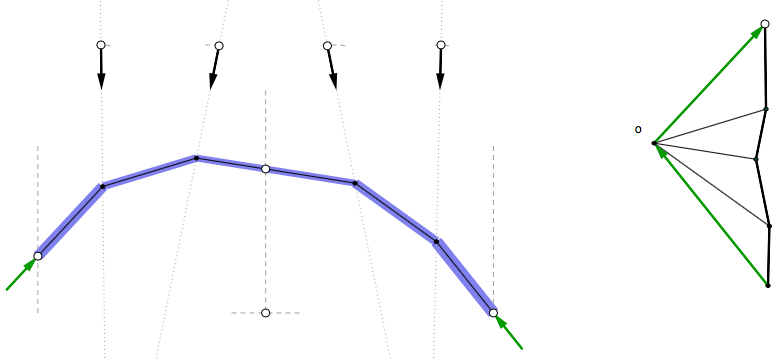
\includegraphics[width=330pt]{graphics/equilibrium.png}
  \caption{The interactive graphic statics software Equilibrium \cite{Block}}
  \label{fig:equilibrium}
\end{figure}

Multiple graphic static computational design tools have been developed; they make use of graphic statics simplicity that allows the computations to run in real-time. The first such application that was developed such application is ActiveStatics \cite{ActiveStatics}, a web-based tool that allows the user to explore graphic statics. Focus of the tool is teaching how graphic statics works, and extensive examples are available. A very similar version named Equilibrium \cite{Block} was later developed, see Figure \ref{fig:equilibrium}. Another similar design tool that instead makes use of particle-spring system for computations is CADenary \cite{CADenary}.


\subsection{Interactive optimization design tools}

\begin{figure}
  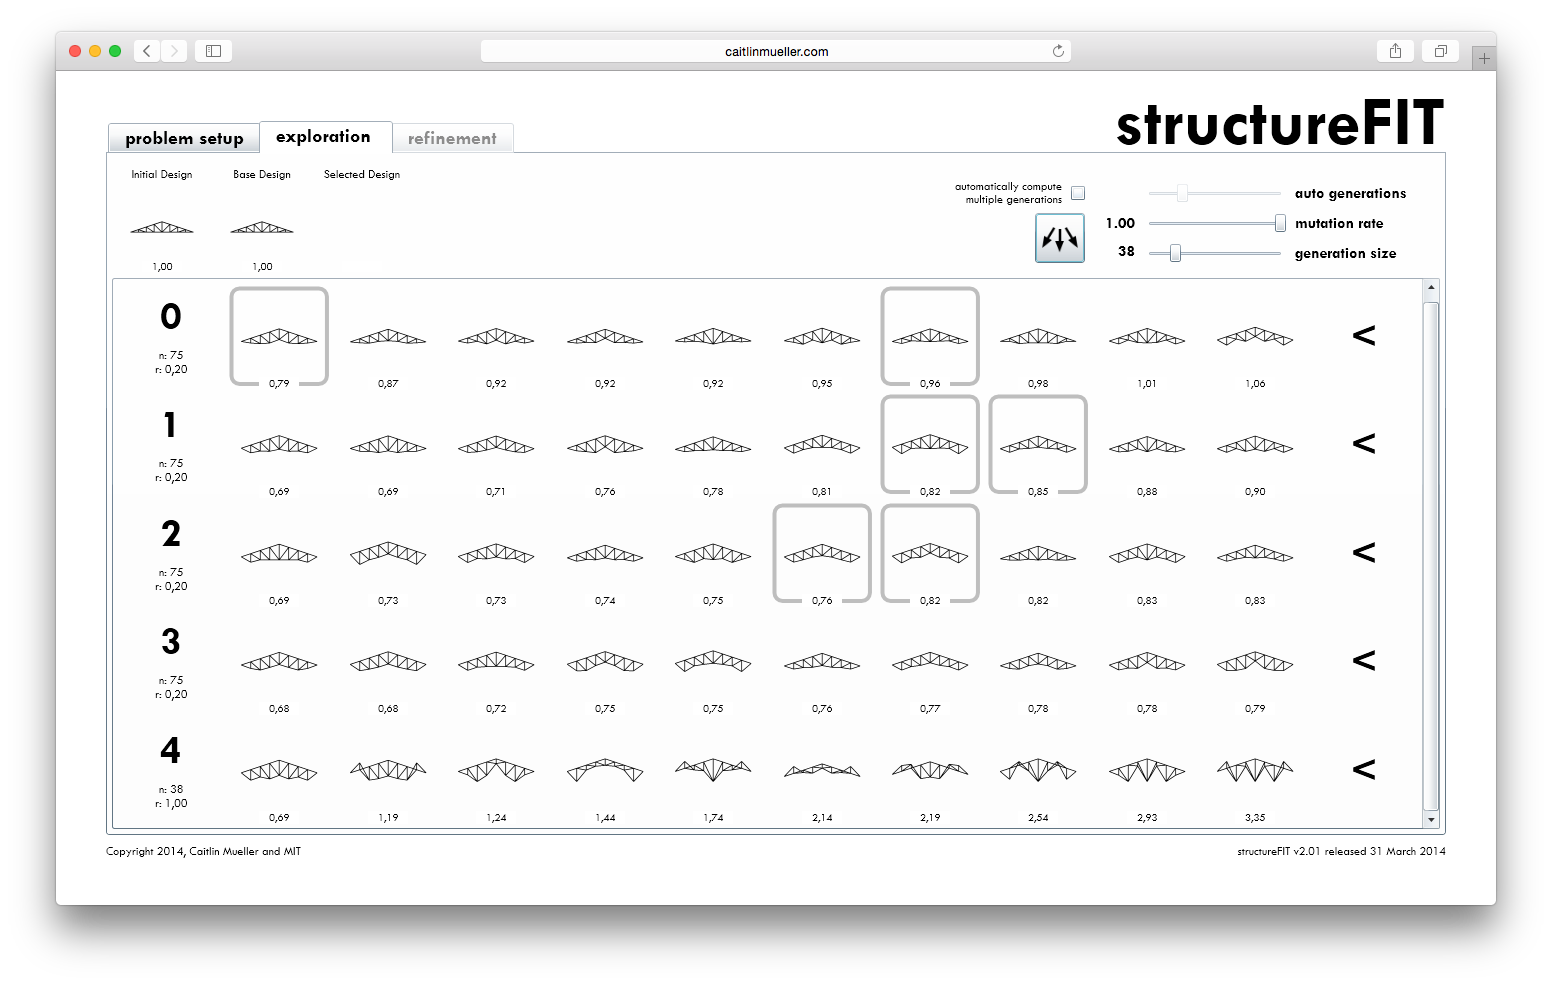
\includegraphics[width=350pt]{graphics/structurefit.png}
  \caption{Screenshot of StructureFIT}
  \label{fig:structurefit}
\end{figure}

Genetic algorithm can easily be used for interactive optimization, where the user can intervene the selection process and direct the population in a desired direction. Such applications have been developed for conceptual structural design, to generate and analyze structures such as bridges and trusses. One such tool is von Buelow’s interactive evolutionary design tool \cite{VonBuelow2008}, which has support for both 2D and 3D structures.

Another similar application, developed as a web application, is named StructureFIT \cite{Mueller2013, Mueller2015}, see Figure \ref{fig:structurefit}. The software tool also has a direct manipulation mode where the user can further explore a generated structure by moving nodes and in real-time see how a relative performance index is updated. Another version of this tool has been developed for Grasshopper \cite{Grasshopper}, named Stormcloud \cite{Danhaive2015}.

\subsection{Topology optimization design tools}
Two other applications that were developed in academia for design exploration through the use of topology optimization are ForcePad (see Figure \ref{fig:forcepad}) \cite{Lindemann2004} and TopOpt \cite{Aage2013}. In the two applications a 2D geometry is modeled by use of conventional drawing tools, a metaphor for “drawing with stiffness”. A topology optimization is then performed on the geometry and the resulting optimized shape is visualized. The applications also have an interactive mode where forces can be manipulated, and the resulting stresses updated in real-time.

\begin{figure}
  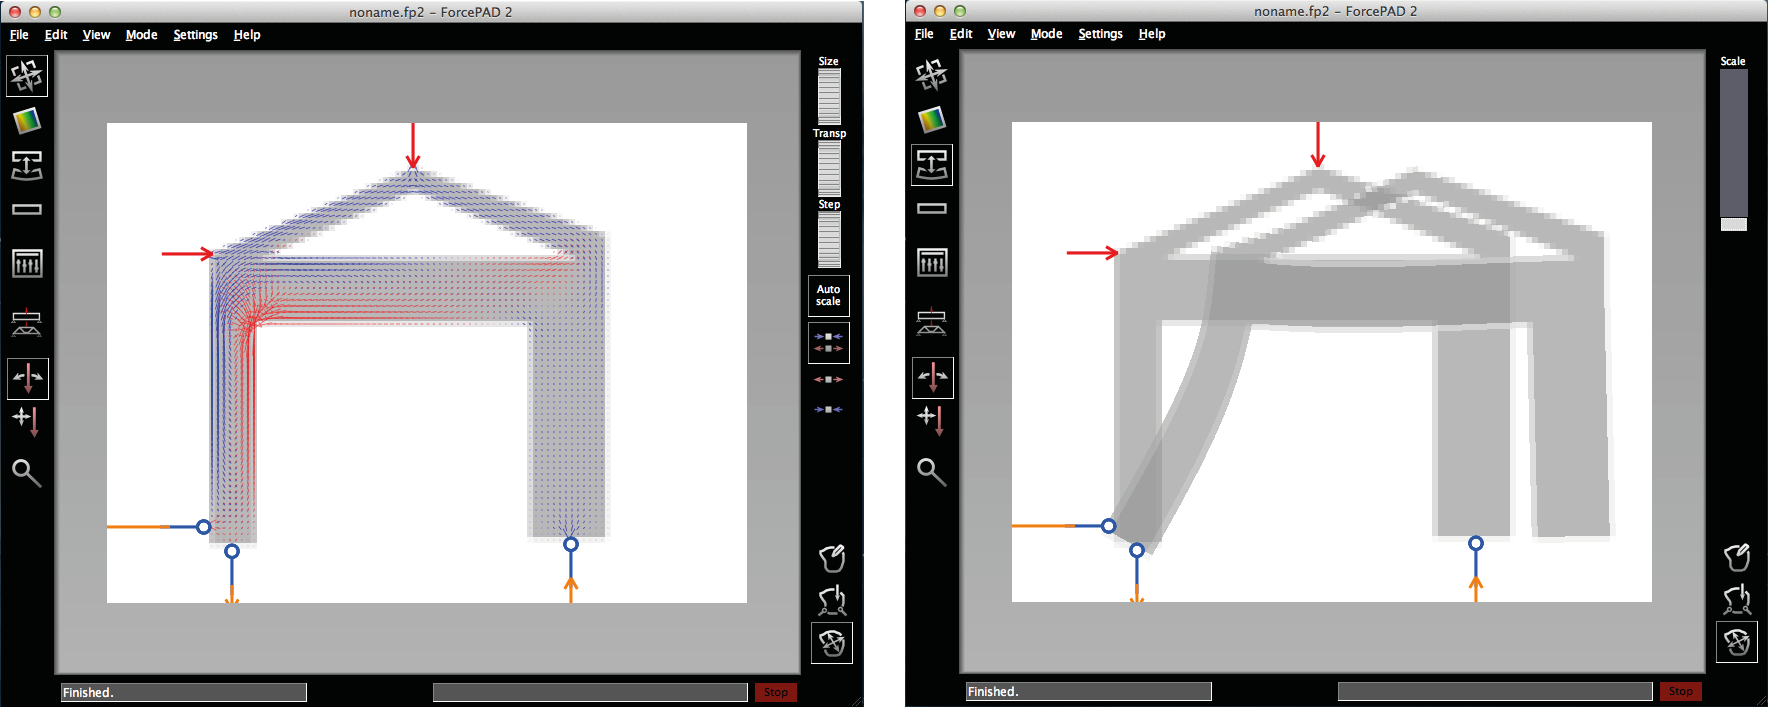
\includegraphics[width=350pt]{graphics/forcepad.png}
  \caption{Software tool ForcePad}
  \label{fig:forcepad}
\end{figure}
